%% This is an example first chapter.  You should put chapter/appendix that you
%% write into a separate file, and add a line \include{yourfilename} to
%% main.tex, where `yourfilename.tex' is the name of the chapter/appendix file.
%% You can process specific files by typing their names in at the 
%% \files=
%% prompt when you run the file main.tex through LaTeX.
\chapter{Use Case 3 - Target-Side Only Input}

\emph{Use case} ini melibatkan hanya satu sisi yaitu \emph{Target-side} saja. pada \emph{use case} ini, input dari salah satu \emph{Target-side} (Protein atau Disease) harus ada.

\section{Protein Search Only}

Pada contoh ini, input dari \emph{Target-side} berupa protein. Contoh ini mencari dari protein yang diinputkan, apa saja senyawa dan penyakit yang terkait dengan protein itu, dan tanaman apa yang dapat menarget protein itu dengan senyawa terkait yang dikandungnya.

\subsection{Input}
\begin{figure}[H]
	\centering
	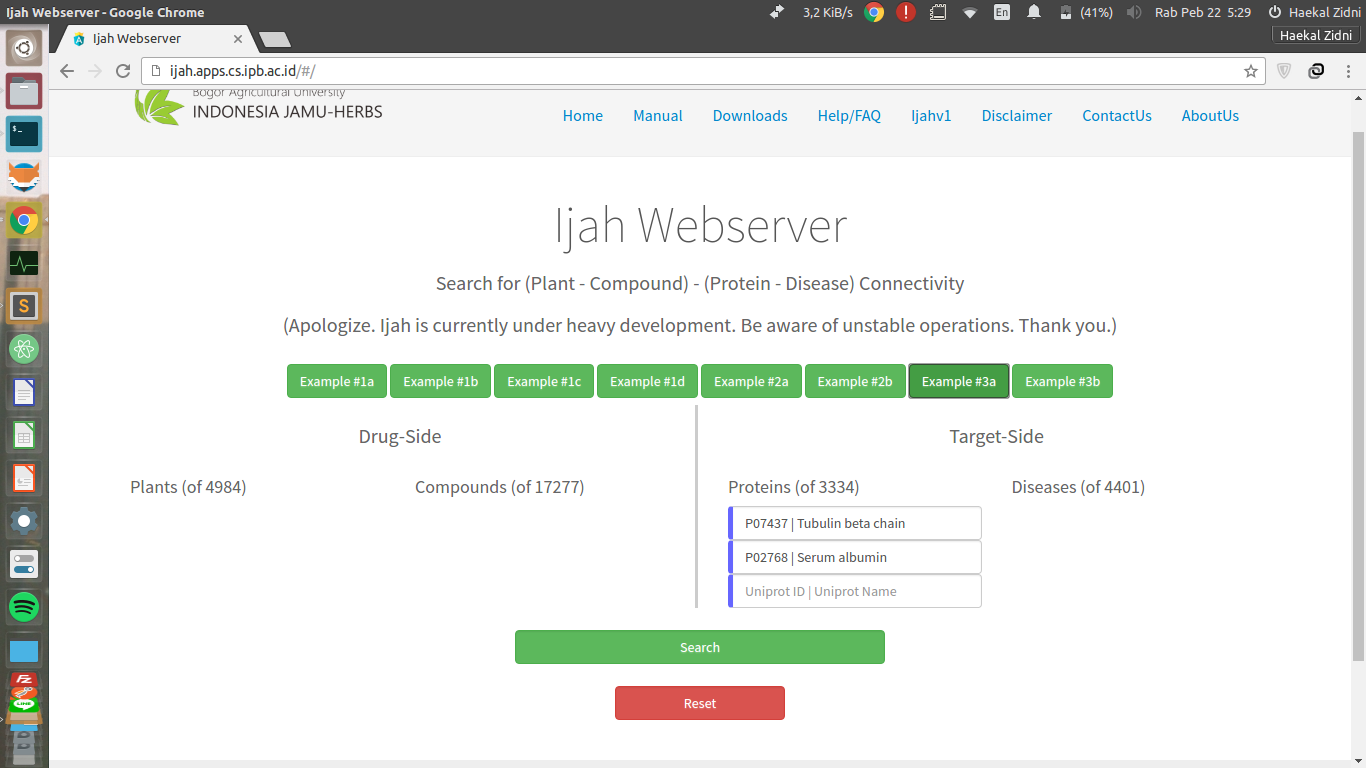
\includegraphics[scale=0.3]{example_3a.png}
	\caption{Contoh \emph{use case} input Protein Search Only}
	\label{fig:example_3a}
\end{figure}

Seperti yang telah dibahas pada bab Use Case 1, untuk jenis \emph{use case} ini tombol hanya bertuliskan \textbf{Search}, bukan Search and Predict seperti \emph{use case} pertama.

\subsection{Output}
Output pada contoh \emph{search} dari 2 jenis protein ini adalah sebagai berikut, dimulai dari \emph{Connectivity Graph Output}

\begin{figure}[H]
	\centering
	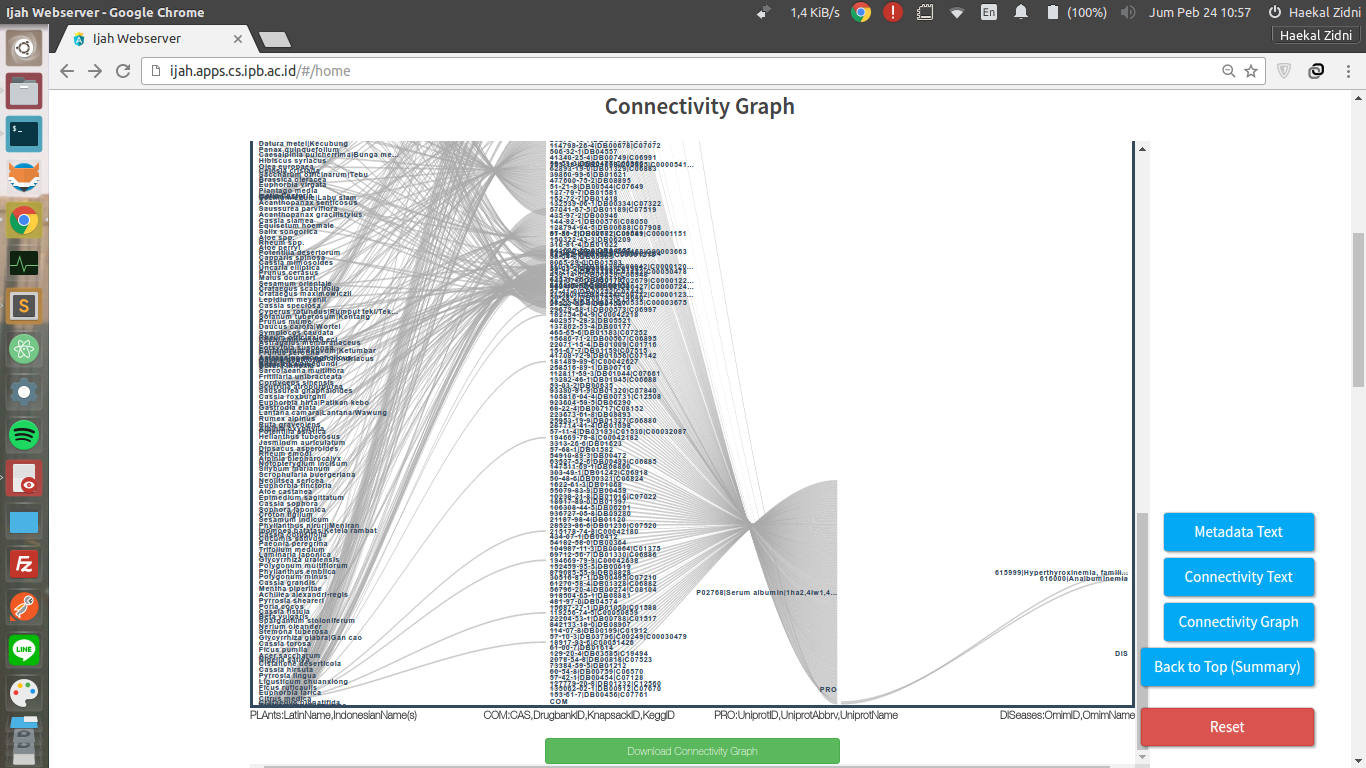
\includegraphics[scale=0.3]{ijah_example_3a_graph.png}
	\caption{Connectivity Graph Output pada use case Protein Search Only}
	\label{fig:ijah_example_3a_output}
\end{figure}

Graf yang dihasilkan kali ini lebih besar lagi karena menampilkan semua senyawa yang terkait dengan protein yang diinputkan, dan dalam contoh ini sangat banyak senyawa yang dapat menarget protein ini. Karena contoh ini menampilkan semua yang terkait dengan protein yang diinputkan.

Hasil \emph{Connectivity Text Output} untuk contoh ini:

\begin{figure}[H]
	\centering
	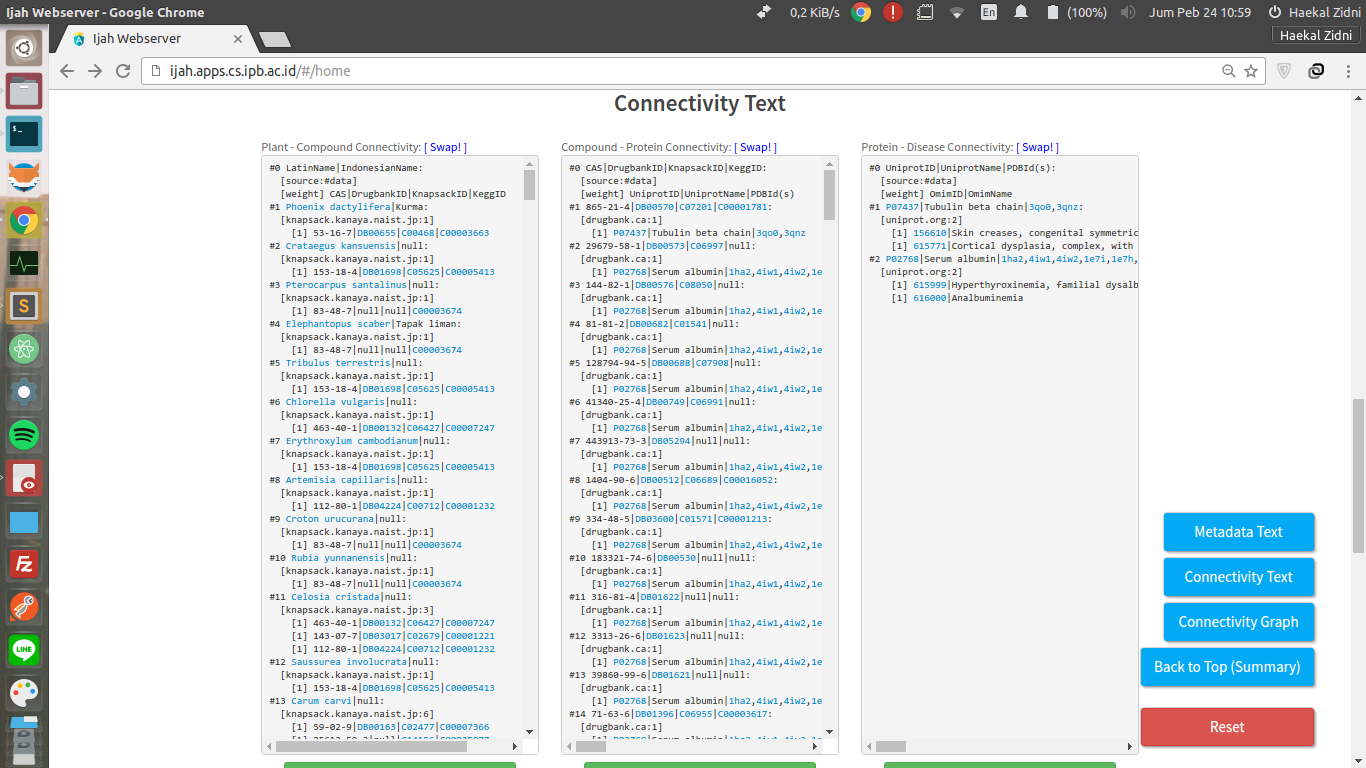
\includegraphics[scale=0.3]{ijah_example_3a_text.png}
	\caption{Connectivity Text Output pada use case Protein Search Only}
	\label{fig:ijah_example_3a_text}
\end{figure}

Hasil \emph{Metadata Text Output} untuk contoh ini:

\begin{figure}[H]
	\centering
	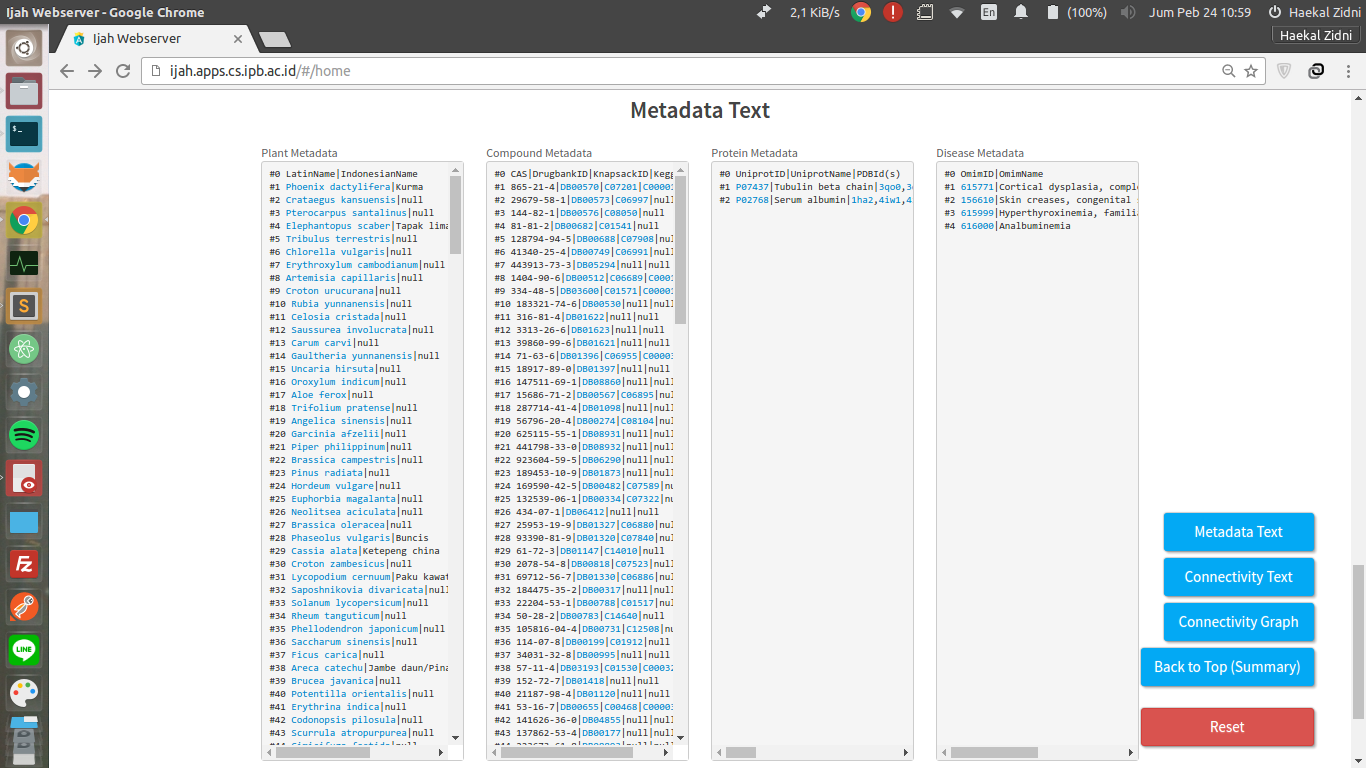
\includegraphics[scale=0.3]{ijah_example_3a_meta.png}
	\caption{Metadata Text Output pada use case Protein Search Only}
	\label{fig:ijah_example_3a_meta}
\end{figure}

\section{Disease Search Only}
Contoh lain dari \emph{use case} Target-Side Only yaitu Disease Search Only dimana perbedaannya hanya pada input, yaitu menginputkan penyakit (Disease) untuk mencari semua (Plant, Compound, Protein) yang terkait dengan penyakit yang diinputkan.



